
\lhead[\chaptername~\thechapter]{\rightmark}


\rhead[\leftmark]{}


\lfoot[\thepage]{}


\cfoot{}


\rfoot[]{\thepage}


\chapter{Messaufbau und -durchf"uhrung}
In diesem Kapitel werden alle Messaufbauten beschrieben und die durchgeführten Messungen erklärt. 

\section{Mechanischer Brustkorb}
In \ref{img:mech-bruskorb} wird der mechanische Brustkorb für die Untersuchung des Versatzes, die Änderung des Winkels über die Frequenz und Einflüsse der Zentripetalkraft auf die Sensoren dargestellt. Da die Schwingprüfanlage \textit{TIRAvib} nur translatorische Schwingungen erzeugen kann, wurde mithilfe eines Holzgestells ein menschlicher Brustkorb imitiert. Dabei werden zwei kurze Balken vertikal an ein Querbalken befestigt, wobei der vordere Balken über ein Scharnier an den Querbalken verbunden ist. Dadurch werden die translatorischen Bewegungen des \textit{TIRAvib} in Rotationsbewegungen umgewandelt. Mithilfe eines Frequenzgenerators kann die Frequenz und Amplitude der Rotationsbewegung eingestellt werden. Durch den Messaufbau können Atemfrequenzen und Brustkorbauslenkungen simuliert und für Charakterisierungs- und Kalibrierungszwecke eingesetzt werden.

\begin{figure}
	\centering
	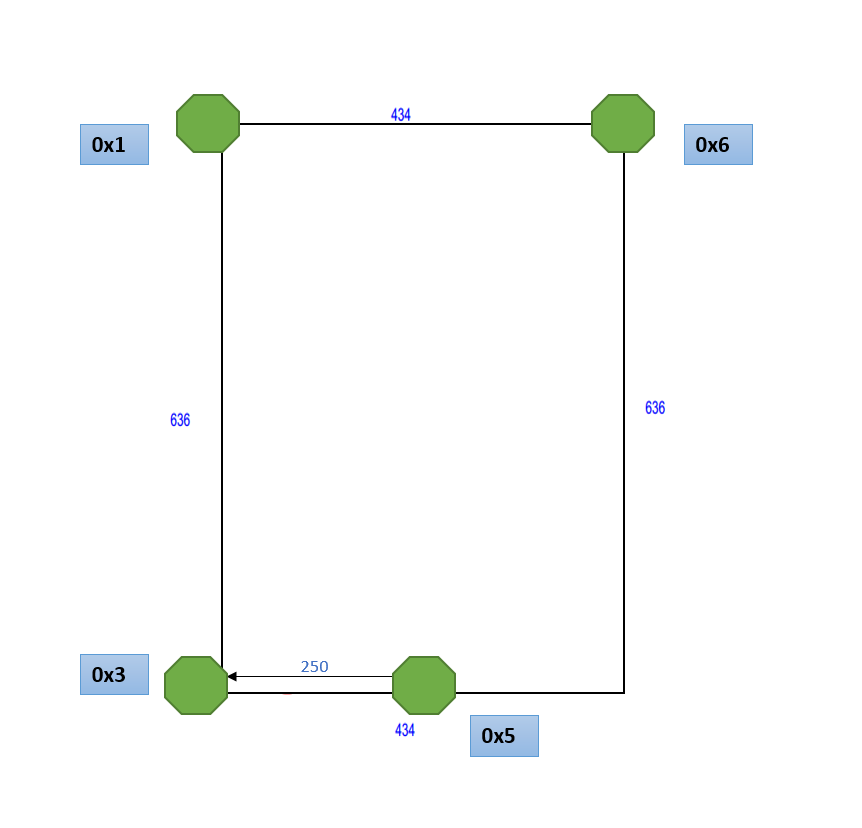
\includegraphics[width=0.35\textwidth]{images/mechBrustkorb}
	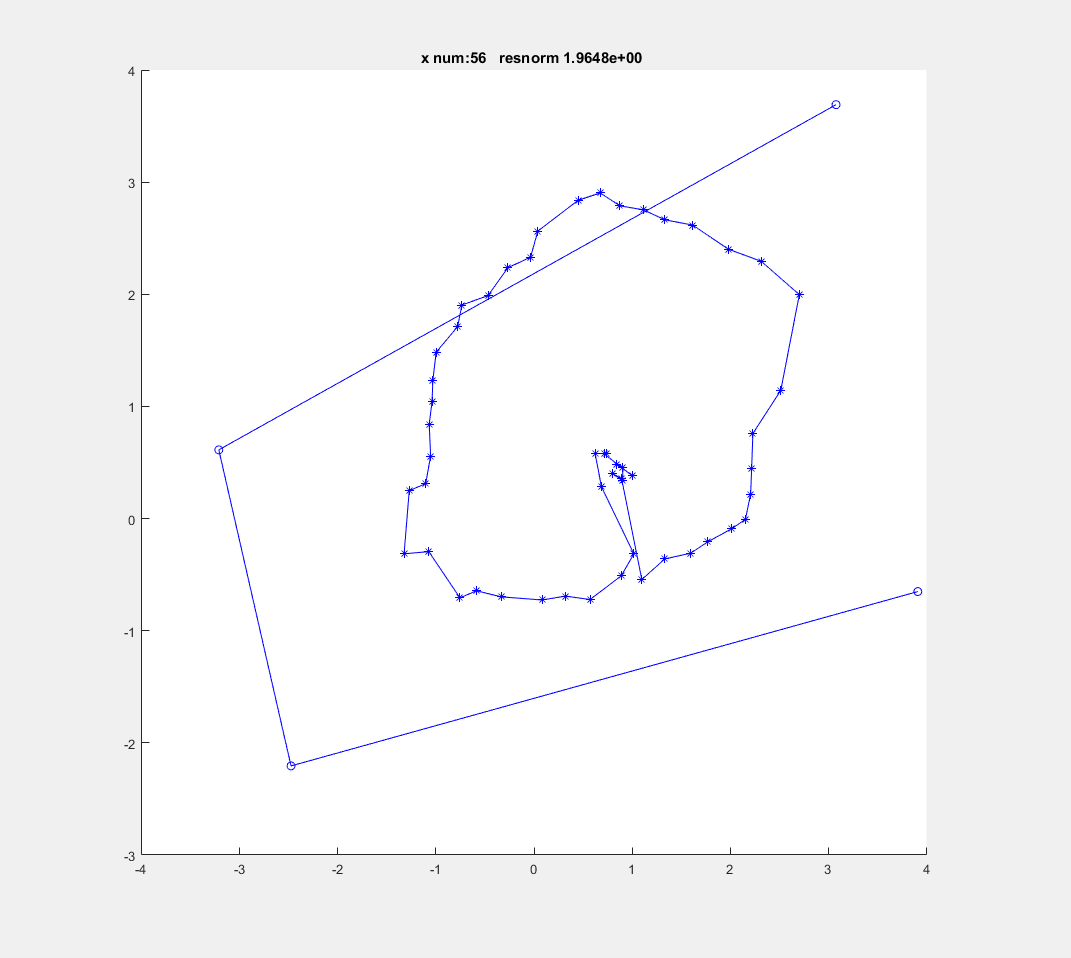
\includegraphics[width=0.38\textwidth]{images/mechBrustkorb2.PNG}
	\caption[Mechanischer Brustkorb]{Mithilfe einer Schwingprüfanlage und einem Gestell aus Holz wird ein mechanischer Brustkorb für die Imitation der Atemfrequenz und Brustkorbauslenkung gebaut.}
	\label{img:mech-bruskorb}
\end{figure}

	\subsection{Versatz}
	Der Versatz gibt an, wie groß der Abstand zwischen den Messwerten der gleichen Zeiteinheit ist. Da die Daten vom Sensor zum Mikrocontroller über die serielle SPI-Schnittstelle übertragen wird und außerdem der Mikrocontroller die Daten sequentiell abfragt, muss der Versatz bekannt sein, um asynchrone Überlagerungen in der Signalverarbeitung zu vermeiden. \ref{img:versatz} illustriert beispielhaft, wie der Versatz zwischen zwei Signalen entsteht.
	
	\begin{figure}[h]
		\centering
		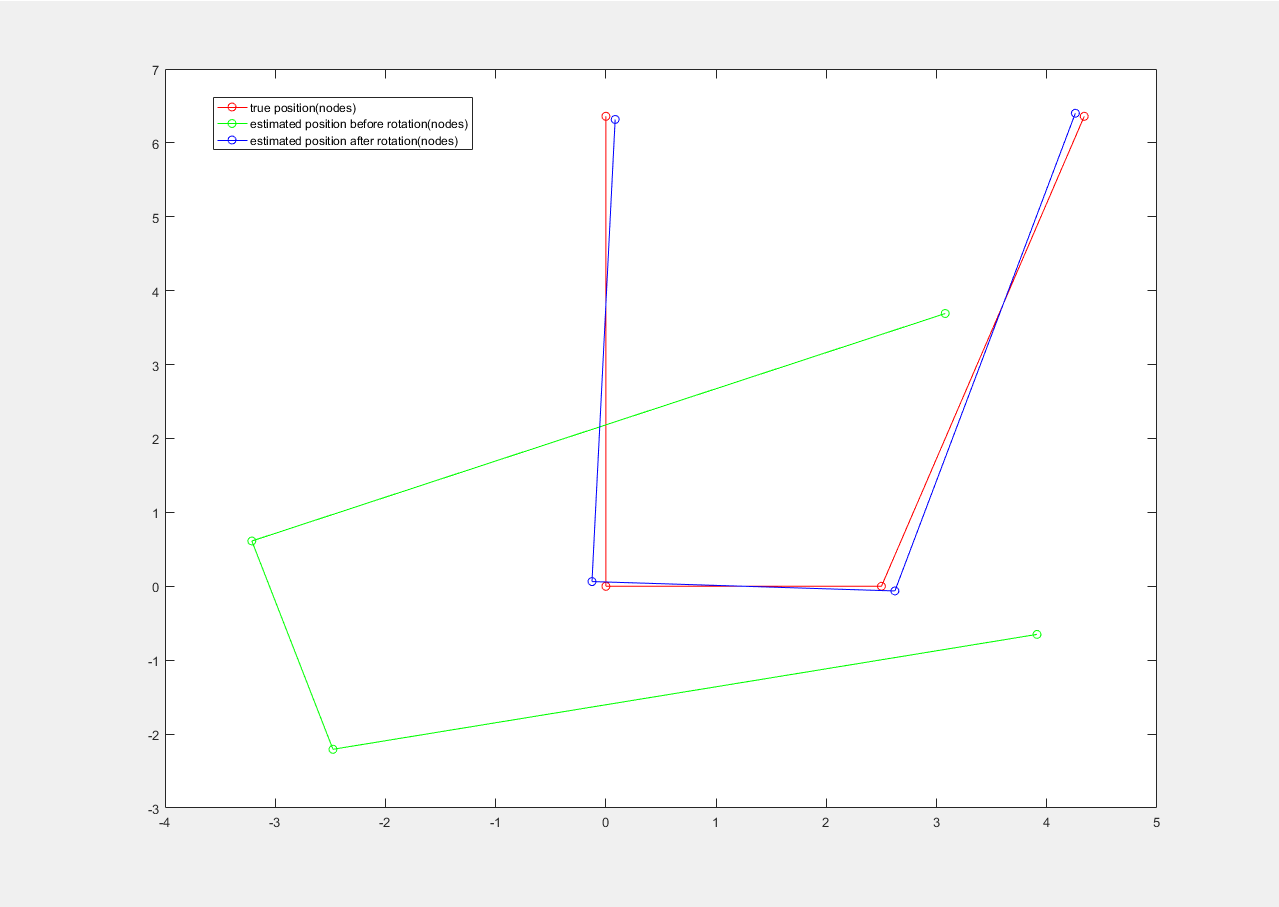
\includegraphics[width=0.7\textwidth]{images/versatz.PNG}
		\caption[Versatz zwischen zwei Signalen]{Aufgrund der sequentiellen Erfassung von Sensor und Mikrocontroller erfährt das blaue Signal eine Verschiebung um t$_\text{v}$.}
		\label{img:versatz}
	\end{figure}

	Für die Versatzmessung werden Brust- und Rückenplatine an dem vorderen Balken des mechanischen Brustkorbs befestigt, sodass sie die gleiche Schwinungung erhalten. und mit einer Frequenz von 100~Hz und einer Amplitude von 50~mV am Frequenzgenerator betrieben. Daraus resultiert eine hochfrequente Vibration, mit sehr spitzen Amplituden. Für die Versatzmessung wird die Abtastrate der Sensoren auf 1~kHz gesetzt, um möglichst viele Messpunkte zu erhalten.
	
	\subsection{Winkel pro Frequenz}
	
	\subsection{Zentripetalkr"afte und Erdbeschleunigung}
	
\newpage
	
\section{Kalibrierung}

	\subsection{Kalibrierung an einem Holzbalken}
	
	\begin{figure}[h]
		\centering
		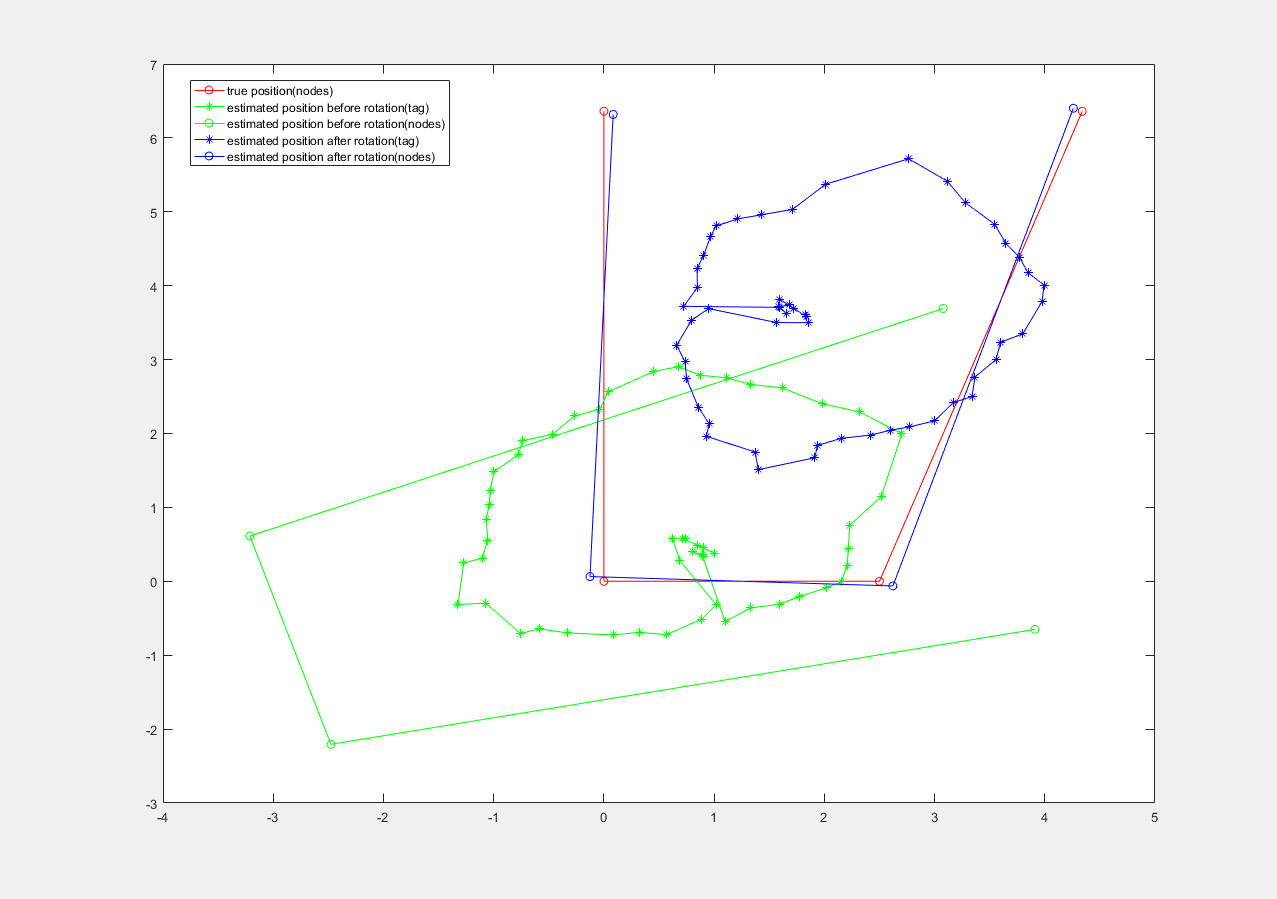
\includegraphics[width=0.5\textwidth]{images/KalibrierungHolzgestell}
		\caption[Kalibrierung an einem Holzbalken]{...}
		\label{img:holzbalken}
	\end{figure}

	\subsection{Vergleich der Kalibrierung mit Referenzsystem}

\newpage

	\subsection{Kalibrierung an einer Testperson}
	
	\begin{figure}[h]
		\centering
		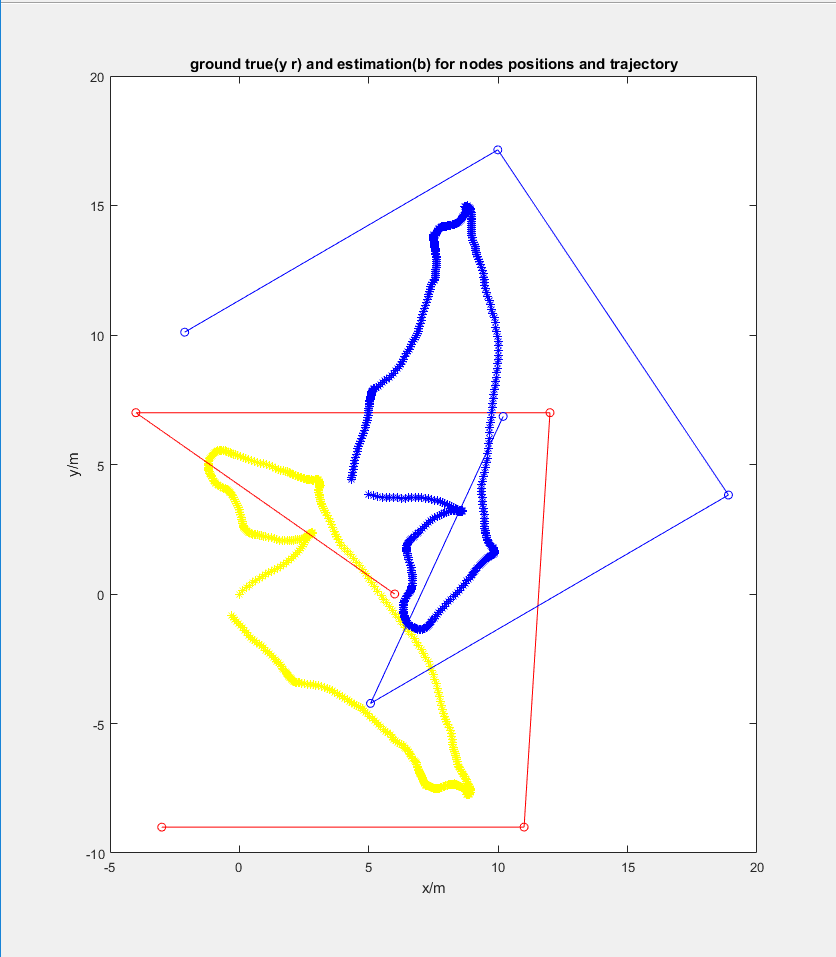
\includegraphics[width=0.5\textwidth]{images/Kalibrierung_Testperson}
		\caption[Kalibrierung an einer Testperson]{...}
		\label{img:testperson}
	\end{figure}